\documentclass{article}

% Language setting
% Replace `english' with e.g. `spanish' to change the document language
\usepackage[english]{babel}

% Set page size and margins
% Replace `letterpaper' with `a4paper' for UK/EU standard size
\usepackage[letterpaper,top=2cm,bottom=2cm,left=3cm,right=3cm,marginparwidth=1.75cm]{geometry}

% Useful packages
\usepackage{amsmath}
\usepackage{graphicx}
\usepackage{float}
\graphicspath{{figure/}}
\usepackage[colorlinks=true, allcolors=blue]{hyperref}
\usepackage{ctex}
\usepackage{listings}
\usepackage{color}
\usepackage{xcolor}
\definecolor{dkgreen}{rgb}{0,0.6,0}
\definecolor{gray}{rgb}{0.5,0.5,0.5}
\definecolor{mauve}{rgb}{0.58,0,0.82}
\lstset{frame=tb,
     language=C++,
     aboveskip=3mm,
     belowskip=3mm,
     showstringspaces=false,
     columns=flexible,
     basicstyle = \ttfamily\small,
     numbers=left,
     numberstyle=\tiny\color{gray},
     keywordstyle=\color{blue},
     commentstyle=\color{dkgreen},
     stringstyle=\color{mauve},
     breaklines=true,
     breakatwhitespace=true,
     tabsize=4
}




\title{Homework: xv6 system calls}
\author{刘恒星 2022229044}

\begin{document}
\maketitle

\section{Part One: System call tracing}

第一个任务是要让kernel在每一次系统调用的时候输出调用的函数名和返回值。并且提示去修改syscall.c的syscall()函数

\begin{lstlisting}
void syscall(void)
{
	int num;
	struct proc *curproc = myproc();

	num = curproc->tf->eax;
	if (num > 0 && num < NELEM(syscalls) && syscalls[num])
	{
		curproc->tf->eax = syscalls[num]();
		cprintf("%s -> %d\n", syacall_name[num], curproc->tf->eax);
	}
	else
	{
		cprintf("%d %s: unknown sys call %d\n",
				curproc->pid, curproc->name, num);
		curproc->tf->eax = -1;
	}
}
\end{lstlisting}

可以看出,系统通过$syscall[num]()$来使用系统调用,然后将返回值存回eax中。num会按照规定好的宏定义去映射到预定义的数组下标,通过$static int (*syscalls[])(void) $我们可以知道调用了什么系统调用,并且按照一定顺序将系统调用的函数名存放在一个数组中,最后可以让他输出调用的函数名和返回值。

\begin{lstlisting}
static char *syacall_name[] = {
	[SYS_fork] = "fork",
	[SYS_exit] = "exit",
	[SYS_wait] = "wait",
	[SYS_pipe] = "pipe",
	[SYS_read] = "read",
	[SYS_kill] = "kill",
	[SYS_exec] = "exec",
	[SYS_fstat] = "fstat",
	[SYS_chdir] = "chdir",
	[SYS_dup] = "dup",
	[SYS_getpid] = "getpid",
	[SYS_sbrk] = "sbrk",
	[SYS_sleep] = "sleep",
	[SYS_uptime] = "uptime",
	[SYS_open] = "open",
	[SYS_write] = "write",
	[SYS_mknod] = "mknod",
	[SYS_unlink] = "unlink",
	[SYS_link] = "link",
	[SYS_mkdir] = "mkdir",
	[SYS_close] = "close",
	[SYS_date] = "sys_date",
};

void syscall(void)
{
	int num;
	struct proc *curproc = myproc();

	num = curproc->tf->eax;
	if (num > 0 && num < NELEM(syscalls) && syscalls[num])
	{
		curproc->tf->eax = syscalls[num]();
		cprintf("%s -> %d\n", syacall_name[num], curproc->tf->eax);
	}
	else
	{
		cprintf("%d %s: unknown sys call %d\n",
				curproc->pid, curproc->name, num);
		curproc->tf->eax = -1;
	}
}
\end{lstlisting}

效果如下:
\begin{figure}[H]
    \centering
    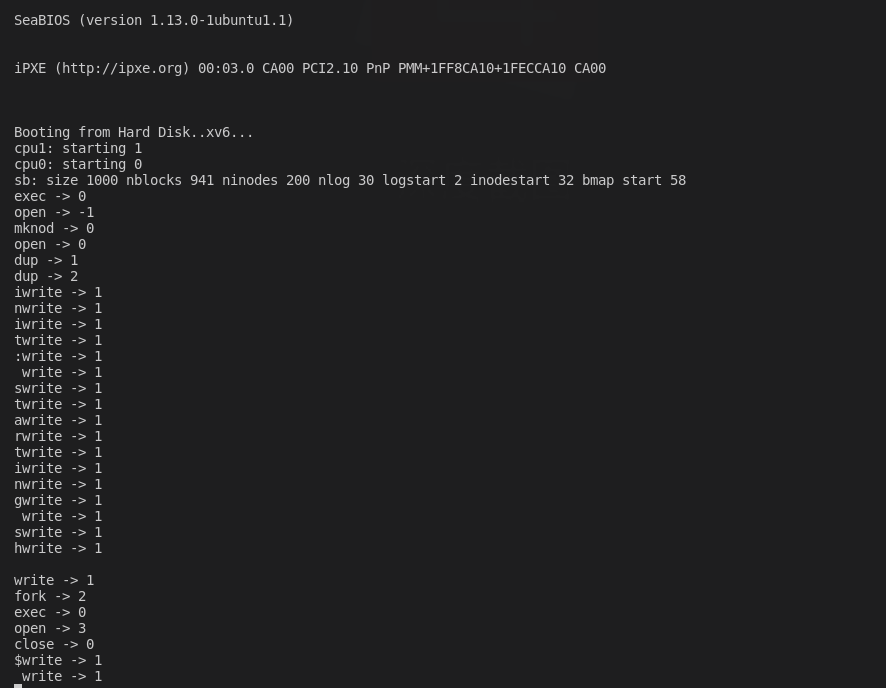
\includegraphics[width=0.9\textwidth]{sys_call.png}
\end{figure} 


\section{Part Two: Date system call}

第二个任务主要是添加一个新的系统调用。任务书中给出了这个调用的源代码的一部分,完善之后如下

\begin{lstlisting}
#include "types.h"
#include "user.h"
#include "date.h"

int main(int argc, char *argv[])
{
	struct rtcdate r;

	if (date(&r))
	{
		printf(2, "date failed\n");
		exit();
	}

	// your code to print the time in any format you like...
	printf(1, "%04d-%02d-%02d  %02d:%02d:%d\n", r.year, r.month, r.day, r.hour, r.minute, r.day);

	exit();
}
\end{lstlisting}

观察rtcdate的结构如下
\begin{lstlisting}
struct rtcdate {
	uint second;
	uint minute;
	uint hour;
	uint day;
	uint month;
	uint year;
};
\end{lstlisting}

可以看出这是一个存放时间的结构体,所以将输出语句写好即可。

接下来是将这个指令变成系统调用,根据任务书做如下步骤

\begin{enumerate}
    \item 在makefile中的UPRGOS添加$_date$
    \item 使用$grep -n uptime *.[chS]$ 指令仿照uptime来补全date缺失的代码
\end{enumerate}

需要注意的是,当我们完成$sysproc.c$的$sys_date()$的时候,可以使用$cmosdate()$函数来获取当前时间,代码如下

\begin{lstlisting}
int sys_date(void)
{
	struct rtcdate *date;
	if (argptr(0, (void *)&date, sizeof(*date)) < 0)
		return -1;
	cmostime(date);
	return 0;
}
\end{lstlisting}

效果如下:
\begin{figure}[H]
    \centering
    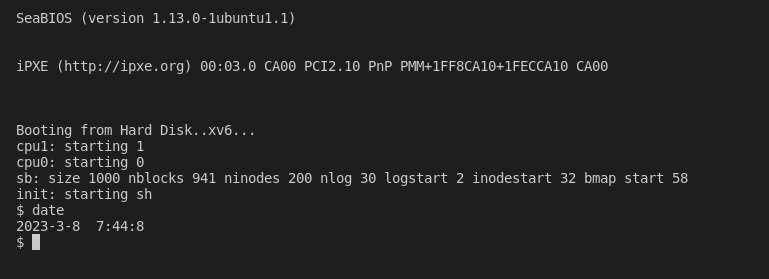
\includegraphics[width=0.9\textwidth]{figure/date_syscall.png}
\end{figure} 


\end{document}